\documentclass{beamer}
\usepackage{ngerman}
% \usepackage{beamerthemelgdv}
\usepackage{./lgdv/beamerthemetest}
\usepackage[T1]{fontenc}
\usepackage[utf8]{inputenc}
\usepackage{subfigure}
\usepackage{listings}

% rough template

\title{Sparse Voxel Octree (SVO) Cone Tracing}
\subtitle{Graphics Project}
\author{Team 2\\P. Kögel, B. Mattes, J. Dörntlein}
\date{\today}

\newcommand{\TODO}[1]{{\large\bf Todo: #1}}

\subject{GraPro}	% goes to pdf meta
\keywords{Computer Graphics, Slides created with LaTeX}	% dito

\begin{document}

\frame{\titlepage}

% \usebackgroundtemplate{}
\newcommand{\slide}[2]{\frame{\frametitle{#1} #2}}
\newcommand{\topic}[1]{\frame{\begin{center}\huge\rm\textbf{#1}\end{center}}}

% \slide{Overview}{
%     \textbf{``Interactive indirect illumination using voxel cone tracing''}
% 	\begin{itemize}
%         \item global illumination approach for game engines in realtime
%         \item fast approximation through voxelization
%         \item rays are bundled to cones -- intersection test with scene voxels
% 	\end{itemize}

%     \begin{figure}[h]
%     \centering
%     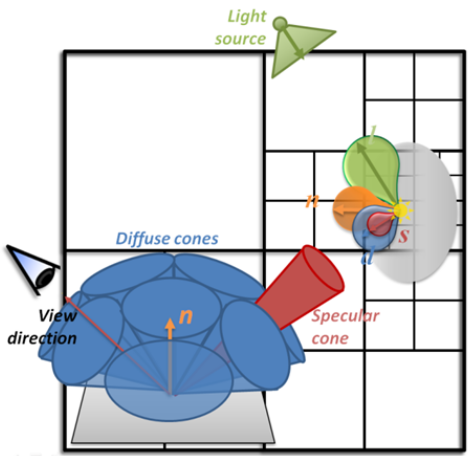
\includegraphics[width=150px]{img/voxel.png}
%     %\caption{Voxel Cone Tracing.}
%     \end{figure}
% }

% \slide{Voxelization}{
%     \begin{itemize}
%         \item equal sized global bounding box is split into grid (eg 256x256x256)
%         \vspace*{5pt}
%         \item voxelization pass:
%     \end{itemize}

%     \vspace*{-15pt}

%     \begin{figure}[h]
%     \centering
%     \includegraphics[width=300px]{img/voxelization.png}
%     %\caption{Voxel Cone Tracing.}
%     \end{figure}
% }

% \slide{Sparse Octree}{
%     \begin{itemize}
%         \item each node is subdivided in 8 subnodes
%         \item only those nodes are filled were the scene is present -> sparse tree
%         \item mipmapping to lower levels
%     \end{itemize}
% }

\slide{Live Demonstration}{
    % some example screenshots here
    Features
    \begin{itemize}
        \item vertex pulling
        \item frustum culling
        \item texturing + normal mapping
        \item GUI
        \item deferred rendering
        \item SMAA
        \item shadow mapping + PCF
        \item emissive + area lights
        \item ambient occlusion
        \item diffuse + specular indirect lighting
    \end{itemize}
}

\end{document}

% vim: set foldmethod=marker foldmarker=[[[,]]]: 


